\appendix
\chapter{Anhang}
\section{Weitere Tabellen}




\section{Ergänzende Abbildungen}

\begin{listing}[h]
\begin{minted}{python}
#pseudocode
class Proc(object):
  def __init__(self, lookup):
    self.lookup = lookup or default_lookup()

  def run(self, step):
    proc = self.lookup[step.stepper](self, step)
    proc.run()
\end{minted}
\caption{Beispiel Zuordnung statt Fabrik}
\label{fig:fabrik-mapping}
\end{listing}


\begin{figure}
    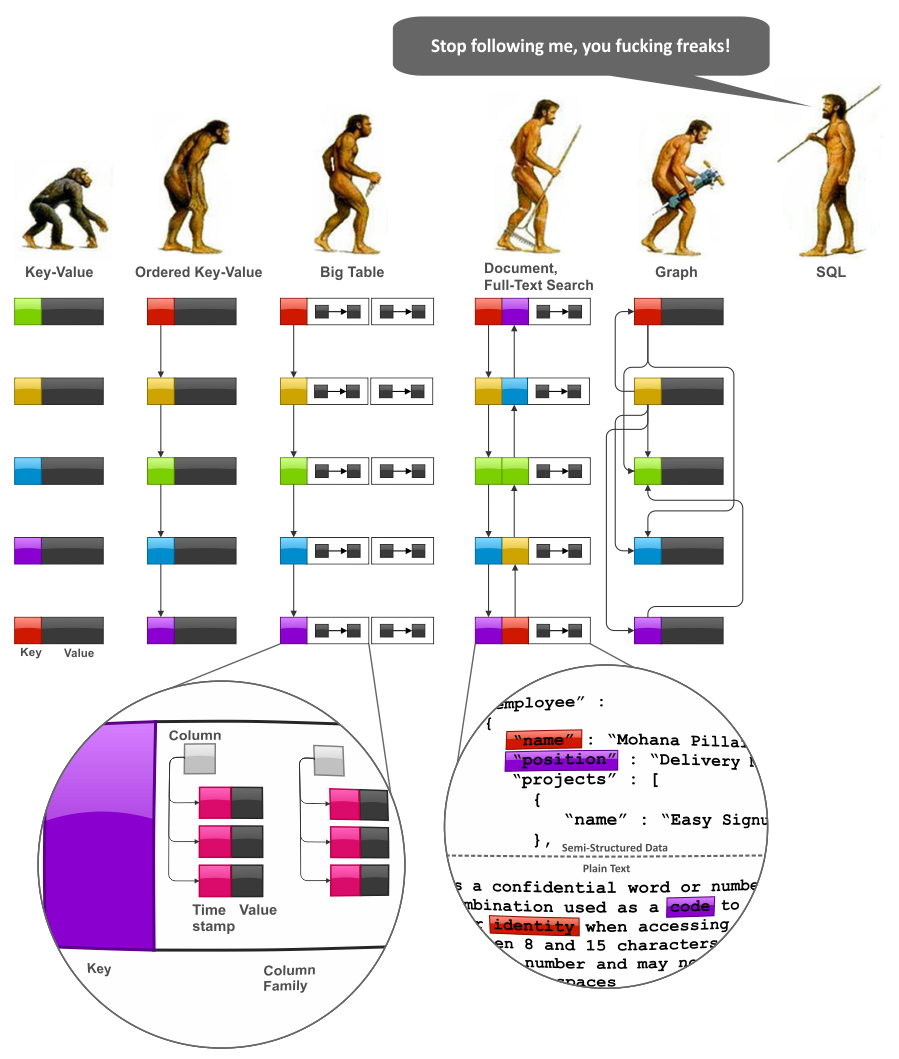
\includegraphics[width=\textwidth]{images/databases-overview.png}
    \caption{Übersicht Klassen an Datenbanken}
    \label{fig:klassen-datenbanken}
\end{figure}
